\section{Implementation}\label{sec:implementation} 

We attempted to generate accurate MPI representations for close-up targets such as heads and upper bodies and improve the pixel accuracies of views synthesized from these MPIs. After putting together the data loader to feed the datasets and point clouds into the network, we recreated loss functions from the textual descriptions in the single-view MPI paper~\cite{single_view_mpi}. As mentioned in subsection~\ref{subsec:base-papers}, we likened our training process to Tucker and Snavely's~\cite{single_view_mpi}, with respect to various aspects such as using TensorFlow 2.2, ADAM solver, a pixel loss weight of 1, a smoothness loss weight of 0.5, etc. We experimented with choices of learning rate and depth loss weight but generally picked 0.00001 and 1, respectively, contrary to the 0.0001 and 0.1 used in Tucker and Snavely. We reduced the learning rate because we were fine-tuning the pretrained model rather than training from scratch. The requirement that we had to have view synthesis quality as supervision was fulfilled by taking frames one frame apart\footnote{in the video sequence} from each chosen training frame as target ground truth. We trained for a certain number of steps rather than for a certain number of epochs. This is because, generally, only smaller/faster-to-train datasets are used for training a model in epochs, whereas it is easier to train larger, indeterminate-in-size datasets in steps. Our data loader randomizes batch picking not only for testing but also for training. Moreover, we have not yet been able to go beyond the model experimentation stage. Exposing the model to a wide variety of frames is the way to go in this stage. For the model to be trained sequentially on all frames clip by clip, covering entire datasets multiple times in multiple epochs, it should be free of any errors that impede its progress toward convergence. We have not been able to bring our model up to that stage yet. 

We used wandb.ai~\cite{wandb} for experiment tracking. It proved to be a valuable tool for our entire process. It helped us spin out different model variants, chiefly characterized by their being trained either on MannequinChallenge alone or on a combination of both datasets. As with some notable attempts at model training in the community, we encountered Not a Number (NaN) gradient errors that took a good chunk of our resolution efforts in this work but ultimately could not be resolved. NaN losses signal that the issue of vanishing/exploding gradients may be present. In this work, NaN gradients could only be reduced in their frequency of occurrence from once in several hundred steps to once in several thousand steps. wandb.ai helped immensely in resuming not just the training runs themselves but also the activity of logging training metrics right from when the run broke off due to a NaN error. What also helped bring down the frequency of encountering NaNs, we believe, was the fact that we removed all those videos from the training/testing process that had at least one frame with a point cloud composed of less than two 3D points. Our Linux command to locate such point cloud \textit{.txt} files (Appendix~\ref{sec:code-snippets}) would take about 3 hours to sift through a set of 2500 point cloud directories with one \textit{.txt} file per video frame. Replacing \textit{cumprod} used in several places in the single-view MPI source code (Figure~\ref{fig:cumprod-model-summary}) with \textit{safe\_cumprod}, as suggested to us by one of the authors of the single-view paper, also helped reduce the frequency of encountering NaNs. One of the issues we could completely resolve was the occasional throwing of \textit{ValueErrors} by our data loader. We also attempted to redress the rendered artifacts mentioned in section~\ref{sec:approach} and determine if real-time, high-quality view synthesis was indeed possible without game engines.

\begin{figure}[!h]
    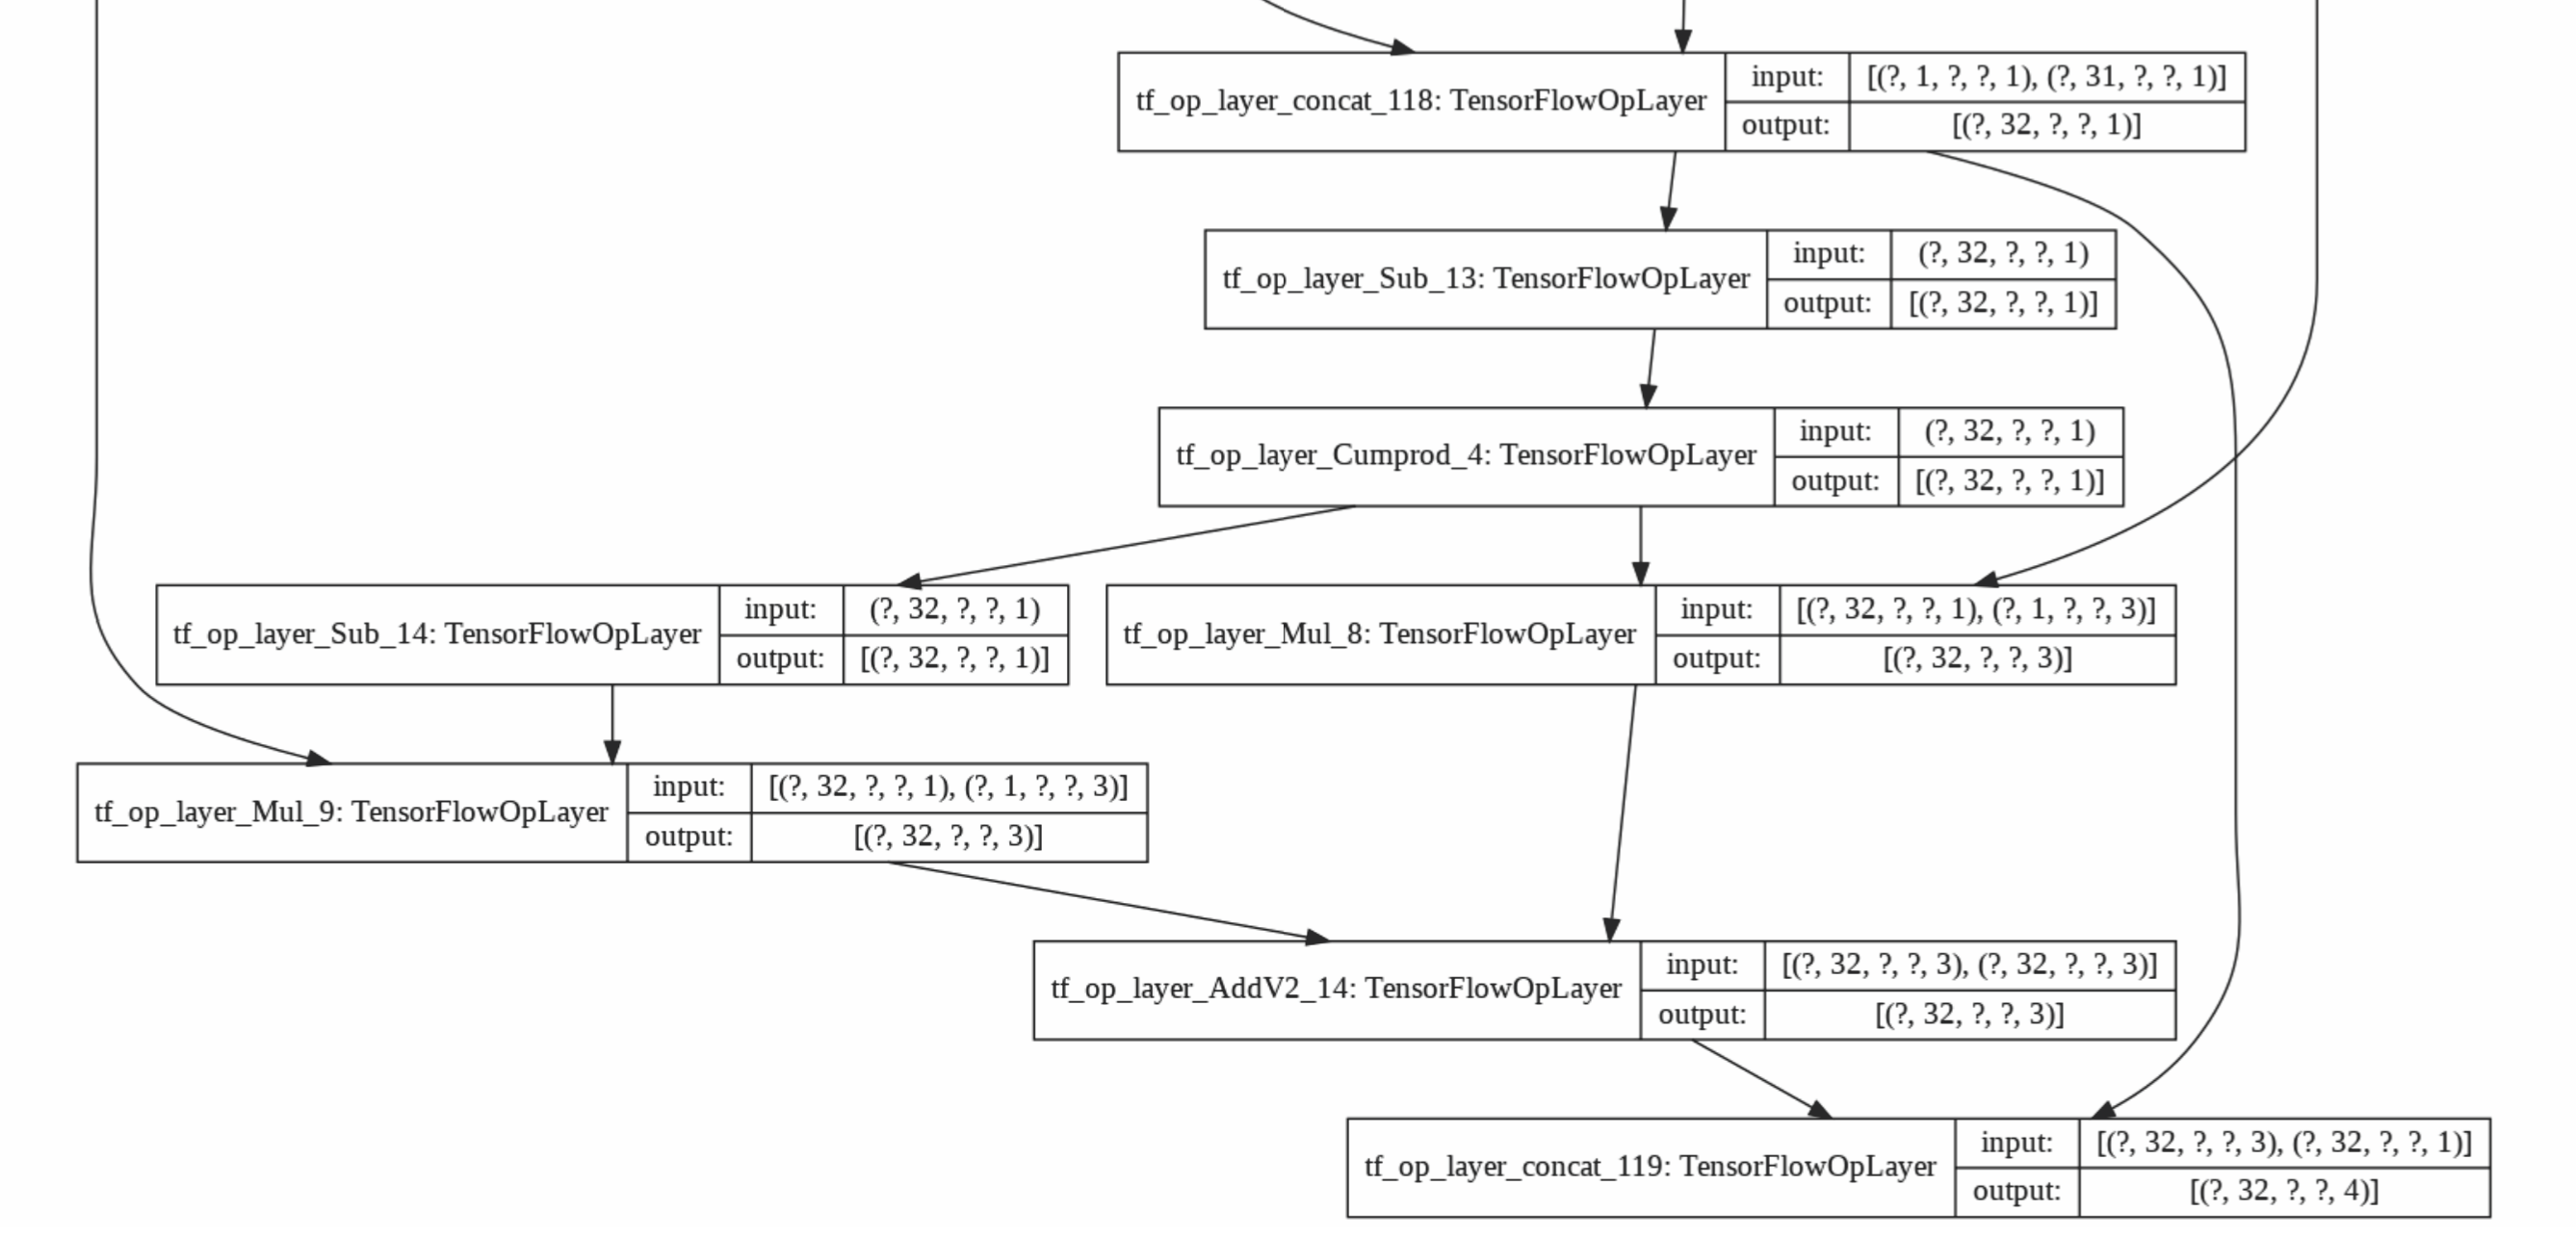
\includegraphics[width=1\columnwidth]{figures/cumprod.png}
    \caption{\textit{Cumprod} Occurring in Single-View MPI Model~\cite{single_view_mpi} as Shown in Google Colaboratory Model Summary}
    \label{fig:cumprod-model-summary}
\end{figure}

We used customized training loops with TensorFlow's \textit{tf.GradientTape} context~\cite{noauthor_custom_nodate}. Nevertheless, we found that the gradient calculation (Appendix~\ref{sec:code-snippets}) would take about a minute! We were using a batch size of 8 on an NVIDIA V100 GPU at the time. The authors of the single-view MPI paper, however, informed us that even on a single worker, their gradient calculation would take less than a second. They then astutely diagnosed our issue to be that we were doing everything in \textit{eager mode}, resulting in excessive overhead. They suggested that using Keras's \textit{model.fit}, using the old estimator system of TensorFlow, or just wrapping things in \textit{tf.function} should allow the critical parts to run in graph mode and be faster. They also suggested that things were probably too big to fit on our GPU. Also, the authors had used a batch size of 4. We ultimately adopted the use of \textit{tf.function} wrapper as well as a batch size of 4 and were able to complete implementing our training and testing pipelines.

\begin{figure}[!h]
    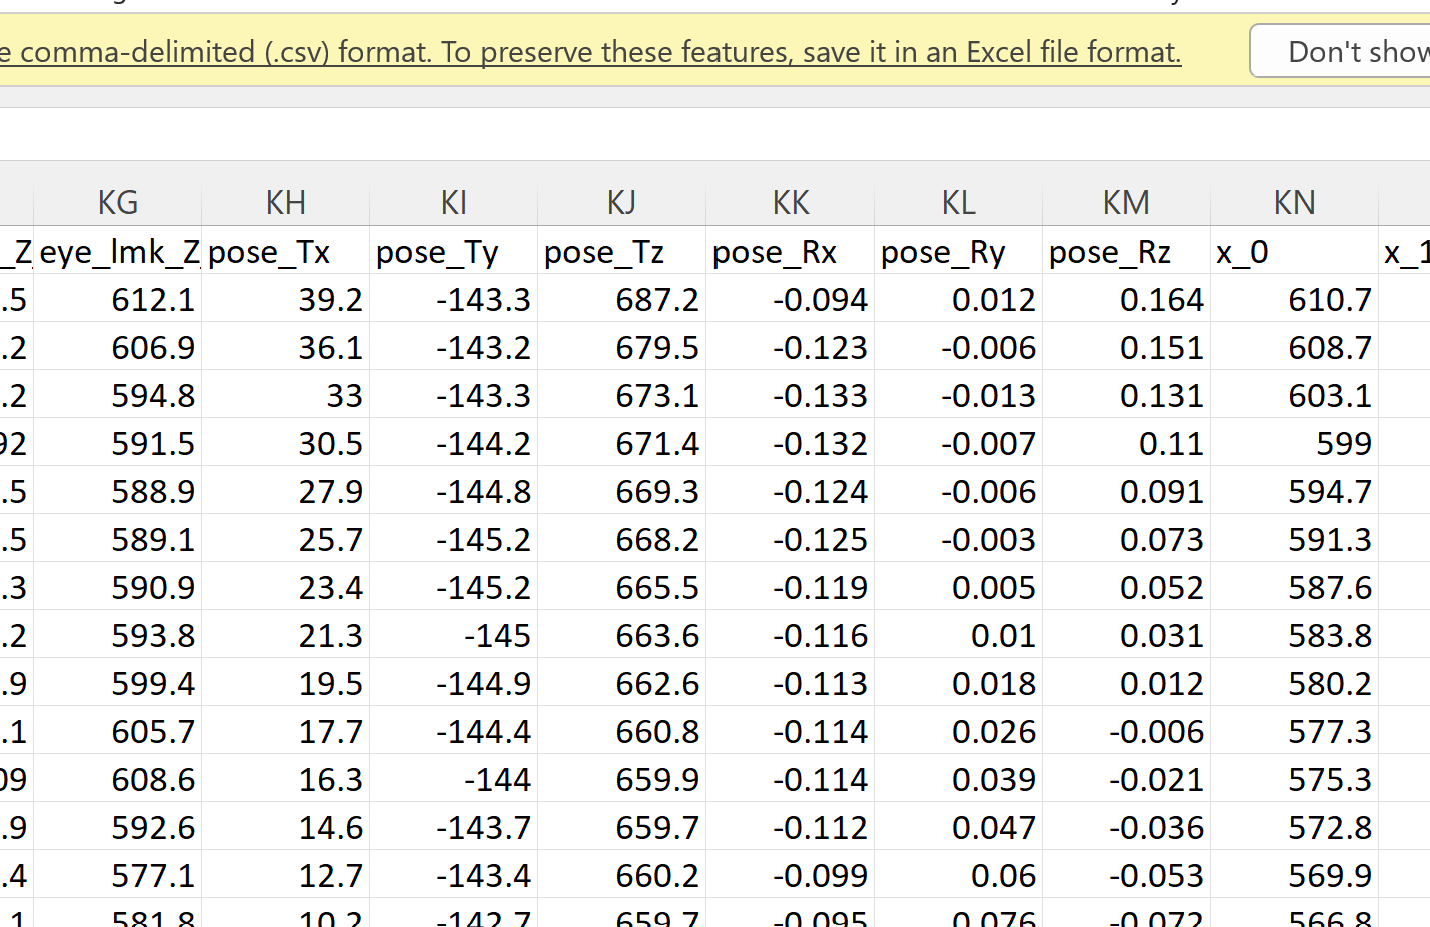
\includegraphics[width=0.75\columnwidth]{figures/openface-csv.png}
    \caption{A Snapshot of OpenFace 2.2~\cite{baltrusaitis_openface_2018} Outputs}
    \label{fig:openface-outputs}
\end{figure}

We then inserted OpenFace 2.2~\cite{baltrusaitis_openface_2018} into the inference pipeline of one of our better-performing model variants and attempted to emulate a video chat system, one half at a time. Using OpenFace 2.2, we extracted the head pose from each frame of a ``viewer" video sequence, as shown in figure~\ref{fig:3d-video-chat-rendering-pipeline}. We used one of the utility functions in the single-view MPI modules, \textit{geometry.pose\_from\_6dof}, to extract the yaw, pitch, and roll angles of the ``viewer" frames in a manner conducive to being accepted by the MPI inference. We then rendered the ``viewee" video sequence at the head pose of the ``viewer" frames with matching timestamps. Even though it looks like more precision could have been added by using not only head pose estimation but also gaze estimation with OpenFace, a compelling argument can be made to the contrary that when we look at people or at a scene, whatever we view does not seem to get ``rerendered" in our visual system based on our changing gaze. It seems to get ``rerendered" based (perhaps solely) on our changing head pose. A snapshot of OpenFace 2.2 outputs for multiple frames in a sequence is shown in figure~\ref{fig:openface-outputs}.